\documentclass[12pt,a4paper]{article}

\usepackage[utf8]{inputenc}
\usepackage[T1]{fontenc}
\usepackage[brazil]{babel}
\usepackage[margin=2.5cm]{geometry}
\usepackage{graphicx}
\usepackage{xcolor}
\usepackage{listings}
\usepackage{amsmath,amssymb}
\usepackage{hyperref}

% ---------------------------------------------------------------------------
% Configuração do listings para código Java com comentários em português
% (acentos via inputenc/T1; o "Delta" de 1042 é tratado via bytes UTF-8 crus
% porque o símbolo grego não é coberto pelo inputenc utf8 padrão)
% ---------------------------------------------------------------------------
\definecolor{codebg}{rgb}{0.96,0.96,0.96}
\definecolor{codegreen}{rgb}{0,0.5,0}
\definecolor{codegray}{rgb}{0.5,0.5,0.5}
\definecolor{codepurple}{rgb}{0.58,0,0.82}

\lstdefinestyle{javastyle}{
    backgroundcolor=\color{codebg},
    commentstyle=\color{codegreen},
    keywordstyle=\color{blue}\bfseries,
    stringstyle=\color{codepurple},
    basicstyle=\ttfamily\footnotesize,
    breakatwhitespace=false,
    breaklines=true,
    captionpos=b,
    keepspaces=true,
    numbers=left,
    numbersep=6pt,
    numberstyle=\tiny\color{codegray},
    showspaces=false,
    showstringspaces=false,
    showtabs=false,
    tabsize=4,
    frame=single,
    language=Java,
    extendedchars=true,
    literate=
        {á}{{\'a}}1 {à}{{\`a}}1 {ã}{{\~a}}1 {â}{{\^a}}1
        {é}{{\'e}}1 {ê}{{\^e}}1
        {í}{{\'i}}1
        {ó}{{\'o}}1 {ô}{{\^o}}1 {õ}{{\~o}}1
        {ú}{{\'u}}1
        {ç}{{\c c}}1
        {Á}{{\'A}}1 {À}{{\`A}}1 {Ã}{{\~A}}1 {Â}{{\^A}}1
        {É}{{\'E}}1 {Ê}{{\^E}}1
        {Í}{{\'I}}1
        {Ó}{{\'O}}1 {Ô}{{\^O}}1 {Õ}{{\~O}}1
        {Ú}{{\'U}}1
        {Ç}{{\c C}}1
        {^^ce^^94}{{$\Delta$}}1
}
\lstset{style=javastyle}

% ---------------------------------------------------------------------------
% Capa
% ---------------------------------------------------------------------------
\title{Trabalho Prático\\\large Fundamentos de Projeto e Análise de Algoritmos (FPA)}
\author{Gustavo Azi Prehl Gama \\ RA: 754737}
\date{\today}

\begin{document}

\maketitle

\section*{Introdução}

Este documento reúne as 10 questões do trabalho prático de FPA, resolvidas
em LeetCode e Codeforces. Para cada questão são apresentados: (i) o código
original submetido; (ii) a cópia integral da tela com a mensagem de aceite
da plataforma; e (iii) uma justificativa de que o código resolve o problema,
fundamentada na teoria de projeto e análise de algoritmos vista em sala
(CLRS09 -- Cormen, Leiserson, Rivest, Stein, \emph{Introduction to
Algorithms}, 3ª ed.).

Em todas as questões, as análises de complexidade de tempo e espaço seguem a
notação assintótica ($O$, $\Theta$, $\Omega$) apresentada em
\emph{Notação Assintótica} [CLRS09, capítulo 3], complementando as
referências específicas de cada estratégia indicadas em cada justificativa.

\tableofcontents
\newpage

\section{392 --- Is Subsequence (LeetCode)}

\subsection*{Código}
\lstinputlisting{392_IsSubsequence.java}

\subsection*{Comprovante de aceite}
\begin{center}
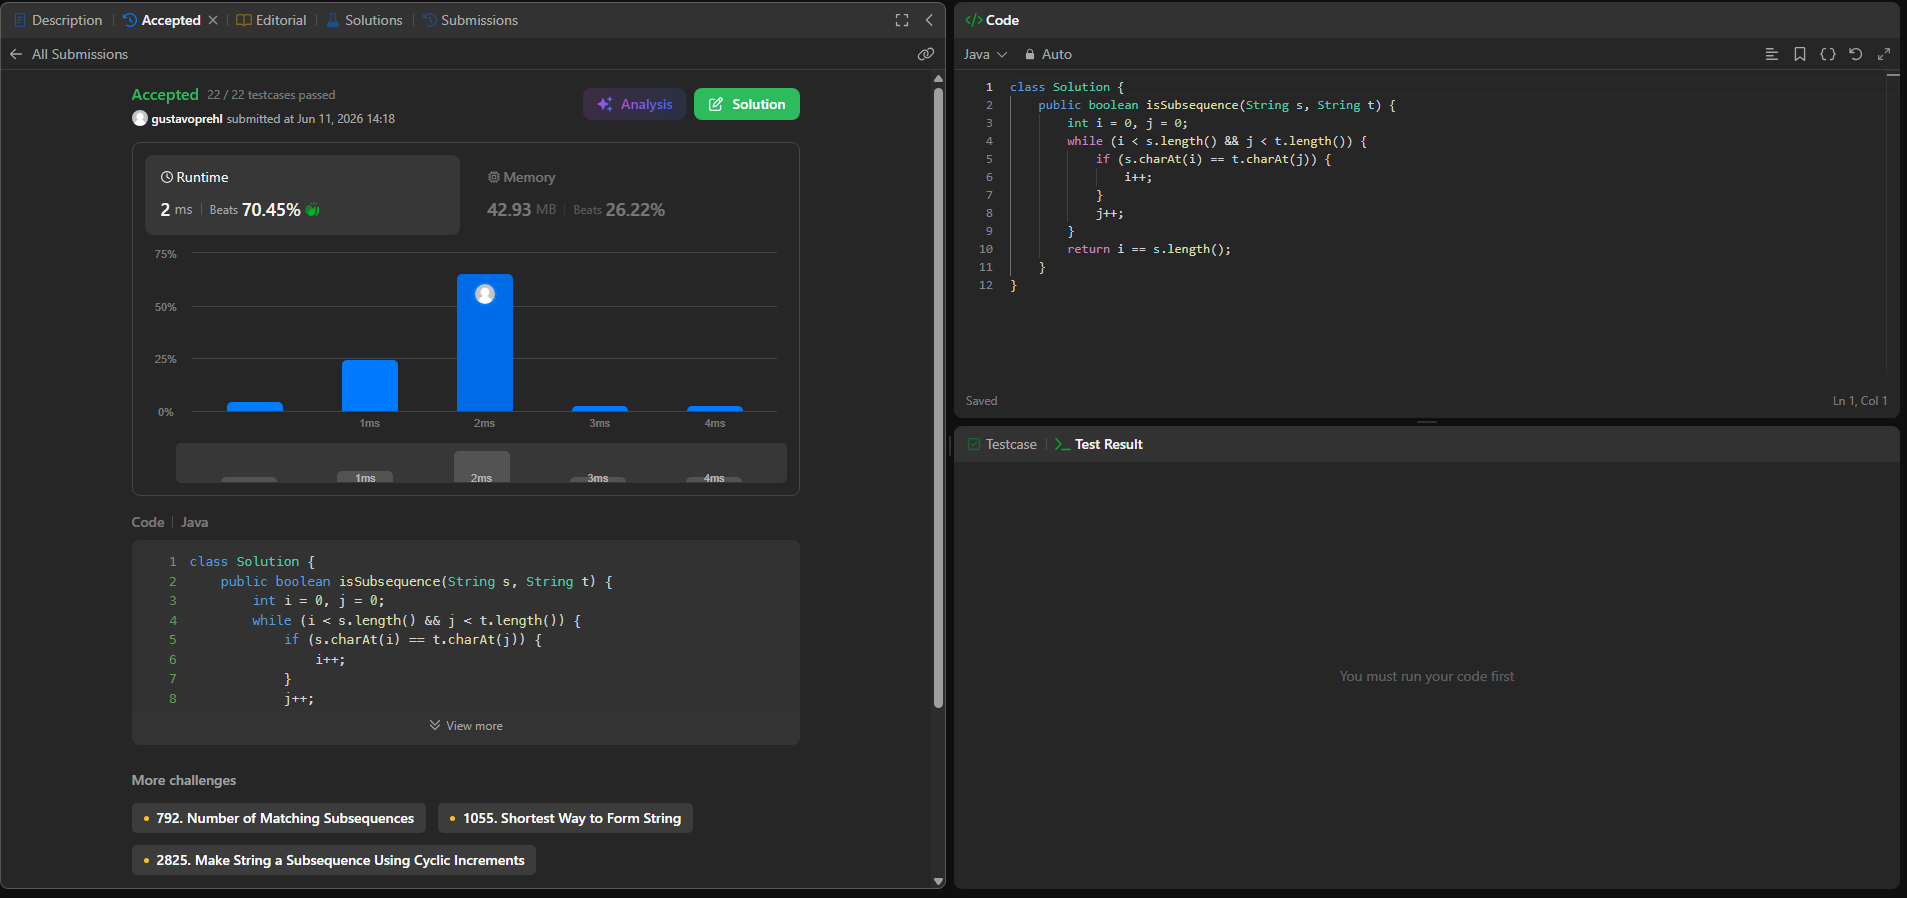
\includegraphics[width=0.85\textwidth]{Accepts/392_IsSubsequence_Submit.png}\\
\end{center}

\subsection*{Justificativa}

\textbf{Estratégia:} dois ponteiros (técnica gulosa).

A solução percorre \texttt{s} (ponteiro \texttt{i}) e \texttt{t} (ponteiro
\texttt{j}) simultaneamente. Sempre que \texttt{s[i] == t[j]}, o caractere de
\texttt{s} é ``consumido'' (\texttt{i++}); o ponteiro \texttt{j} avança a cada
iteração, independentemente de ter havido correspondência. \texttt{s} é
subsequência de \texttt{t} se, ao final, \texttt{i} percorreu todos os
caracteres de \texttt{s}.

\textbf{Por que essa escolha gulosa é ótima (correção):} dado um caractere
\texttt{s[i]} e a primeira ocorrência possível dele em \texttt{t} a partir da
posição \texttt{j}, casar \texttt{s[i]} com essa primeira ocorrência nunca é
pior do que casá-lo com uma ocorrência posterior. Isso porque qualquer
correspondência válida para o restante de \texttt{s} que use uma posição
$j' > j$ também é válida (ou mais restrita) se usarmos $j$, já que sobra mais
``espaço'' em \texttt{t} à direita. Portanto, a escolha gulosa de avançar
assim que há correspondência preserva a existência de uma solução completa,
sem necessidade de backtracking. Esse argumento de troca (\emph{exchange
argument}) é a técnica padrão de prova de corretude de algoritmos gulosos.

\textbf{Complexidade:}
\begin{itemize}
    \item Tempo: $O(|t|)$, pois cada ponteiro avança no máximo $|t|$ vezes.
    \item Espaço: $O(1)$, apenas dois índices inteiros.
\end{itemize}

\textbf{Follow-up ($k \geq 10^9$ consultas sobre o mesmo \texttt{t}):}
pré-processar \texttt{t} uma única vez, construindo, para cada caractere
\texttt{c}, a lista ordenada \texttt{pos[c]} com os índices onde \texttt{c}
ocorre em \texttt{t} --- $O(|t|)$. Para cada nova string $s_i$, percorrer seus
caracteres e, para cada um, fazer busca binária em \texttt{pos[c]} pela menor
posição estritamente maior que a posição atual em \texttt{t}. Se não existir
tal posição para algum caractere, $s_i$ não é subsequência. Isso reduz o
custo por consulta de $O(|t|)$ para $O(|s_i| \cdot \log |t|)$, o que é
essencial quando \texttt{t} é fixo e há um número muito grande de consultas.

\textbf{Tópico do curso:} estratégia gulosa, com prova de corretude por
argumento de troca --- \emph{Estratégia Gulosa e Divisão e Conquista}
[CLRS09, caps. 4 e 16].

\newpage
\section{198 --- House Robber (LeetCode)}

\subsection*{Código}
\lstinputlisting{198_HouseRobber.java}

\subsection*{Comprovante de aceite}
\begin{center}
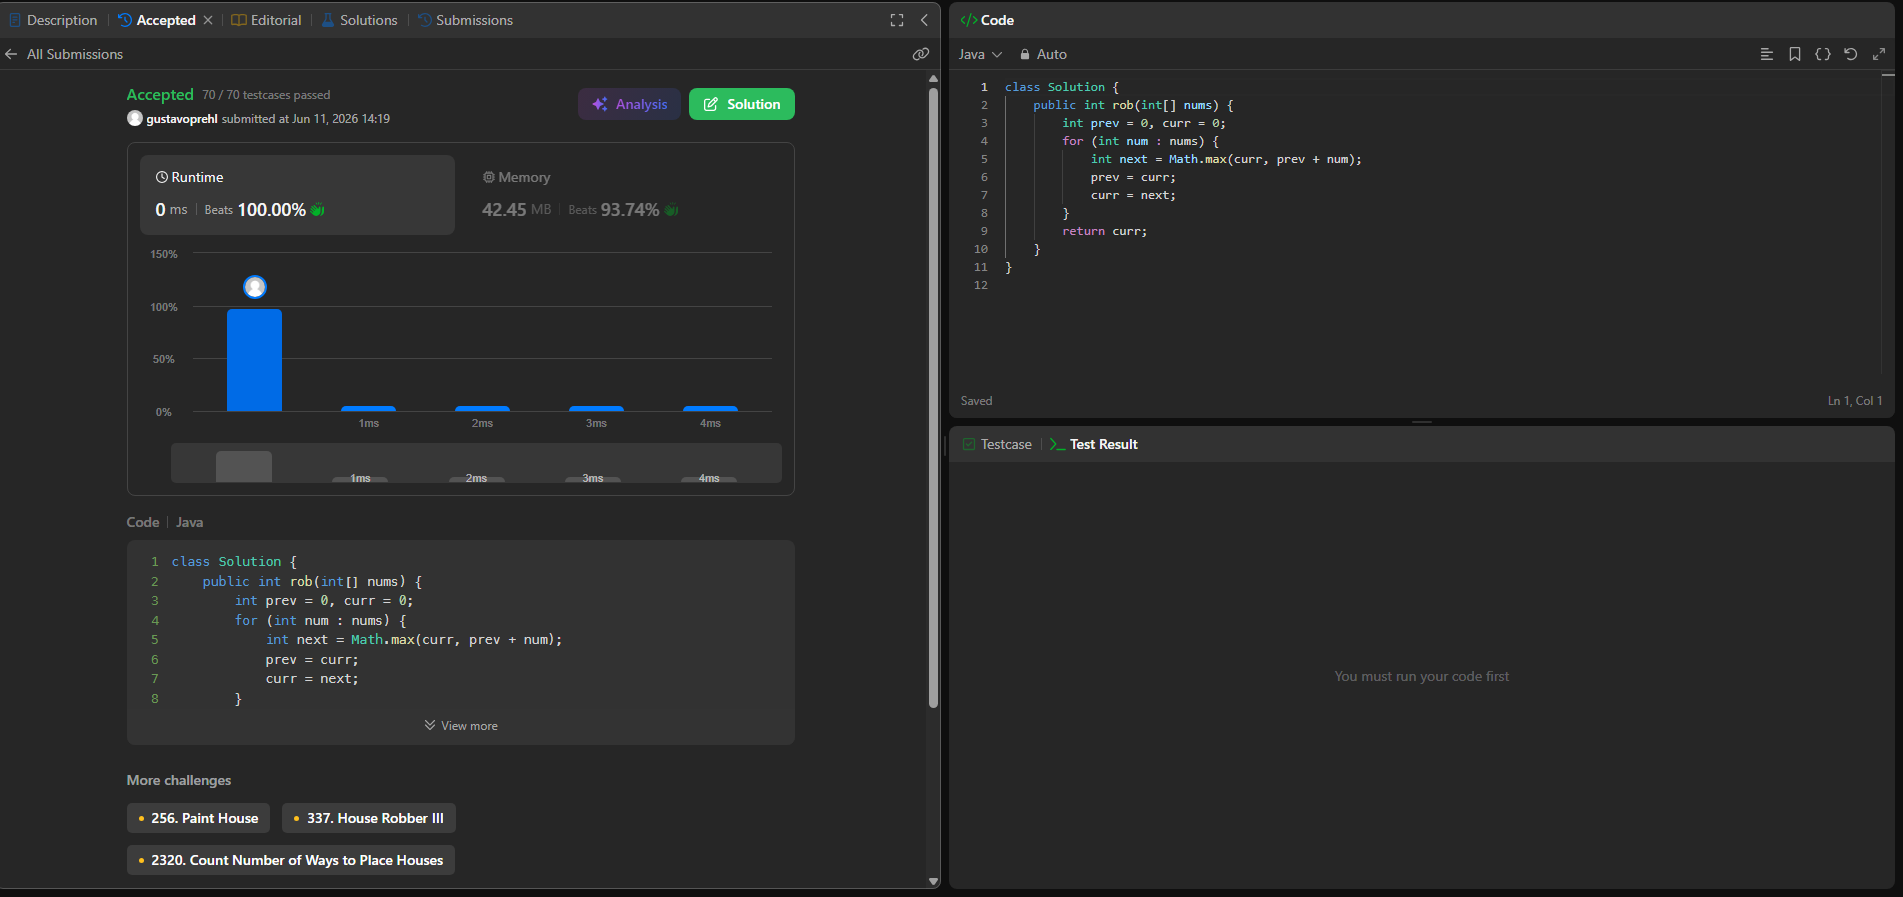
\includegraphics[width=0.85\textwidth]{Accepts/198_HouseRobber_Submit.png}\\
\end{center}

\subsection*{Justificativa}

\textbf{Estratégia:} programação dinâmica (\emph{bottom-up}, com otimização
de espaço).

\textbf{Subestrutura ótima:} seja $dp[i]$ o valor máximo que se pode roubar
considerando apenas as primeiras $i$ casas. Para a casa $i$, há exatamente
duas opções:
\begin{itemize}
    \item \textbf{não roubar a casa $i$}: o melhor valor é $dp[i-1]$;
    \item \textbf{roubar a casa $i$}: como a casa $i-1$ não pode ter sido
    roubada, o melhor valor é $dp[i-2] + nums[i]$.
\end{itemize}

Logo, a recorrência é:
\[
dp[i] = \max\big(dp[i-1],\; dp[i-2] + nums[i]\big)
\]

A solução ótima global é construída a partir das soluções ótimas de
subproblemas menores (prefixos do array), o que caracteriza a propriedade de
\textbf{subestrutura ótima}.

\textbf{Subproblemas sobrepostos:} $dp[i-1]$ e $dp[i-2]$ são reutilizados
repetidamente no cálculo de $dp[i]$, $dp[i+1]$, etc. Em vez de recalcular
esses valores recursivamente (o que levaria a complexidade exponencial), a
abordagem \emph{bottom-up} resolve cada subproblema uma única vez, em ordem
crescente de $i$, armazenando o resultado.

\textbf{Otimização de espaço:} como $dp[i]$ depende apenas dos dois valores
anteriores, não é necessário manter o vetor $dp$ inteiro --- basta guardar
\texttt{prev} ($= dp[i-2]$) e \texttt{curr} ($= dp[i-1]$), atualizando-os a
cada iteração.

\textbf{Complexidade:}
\begin{itemize}
    \item Tempo: $O(n)$, uma única passagem pelo array.
    \item Espaço: $O(1)$, apenas duas variáveis auxiliares.
\end{itemize}

\textbf{Tópico do curso:} \emph{Programação Dinâmica} [CLRS09, cap. 15] ---
identificação de subestrutura ótima e subproblemas sobrepostos, com
formulação da recorrência \emph{bottom-up} e otimização do espaço de
armazenamento.

\newpage
\section{1042 --- Flower Planting With No Adjacent (LeetCode)}

\subsection*{Código}
\lstinputlisting{1042_FlowerPlanting.java}

\subsection*{Comprovante de aceite}
\begin{center}
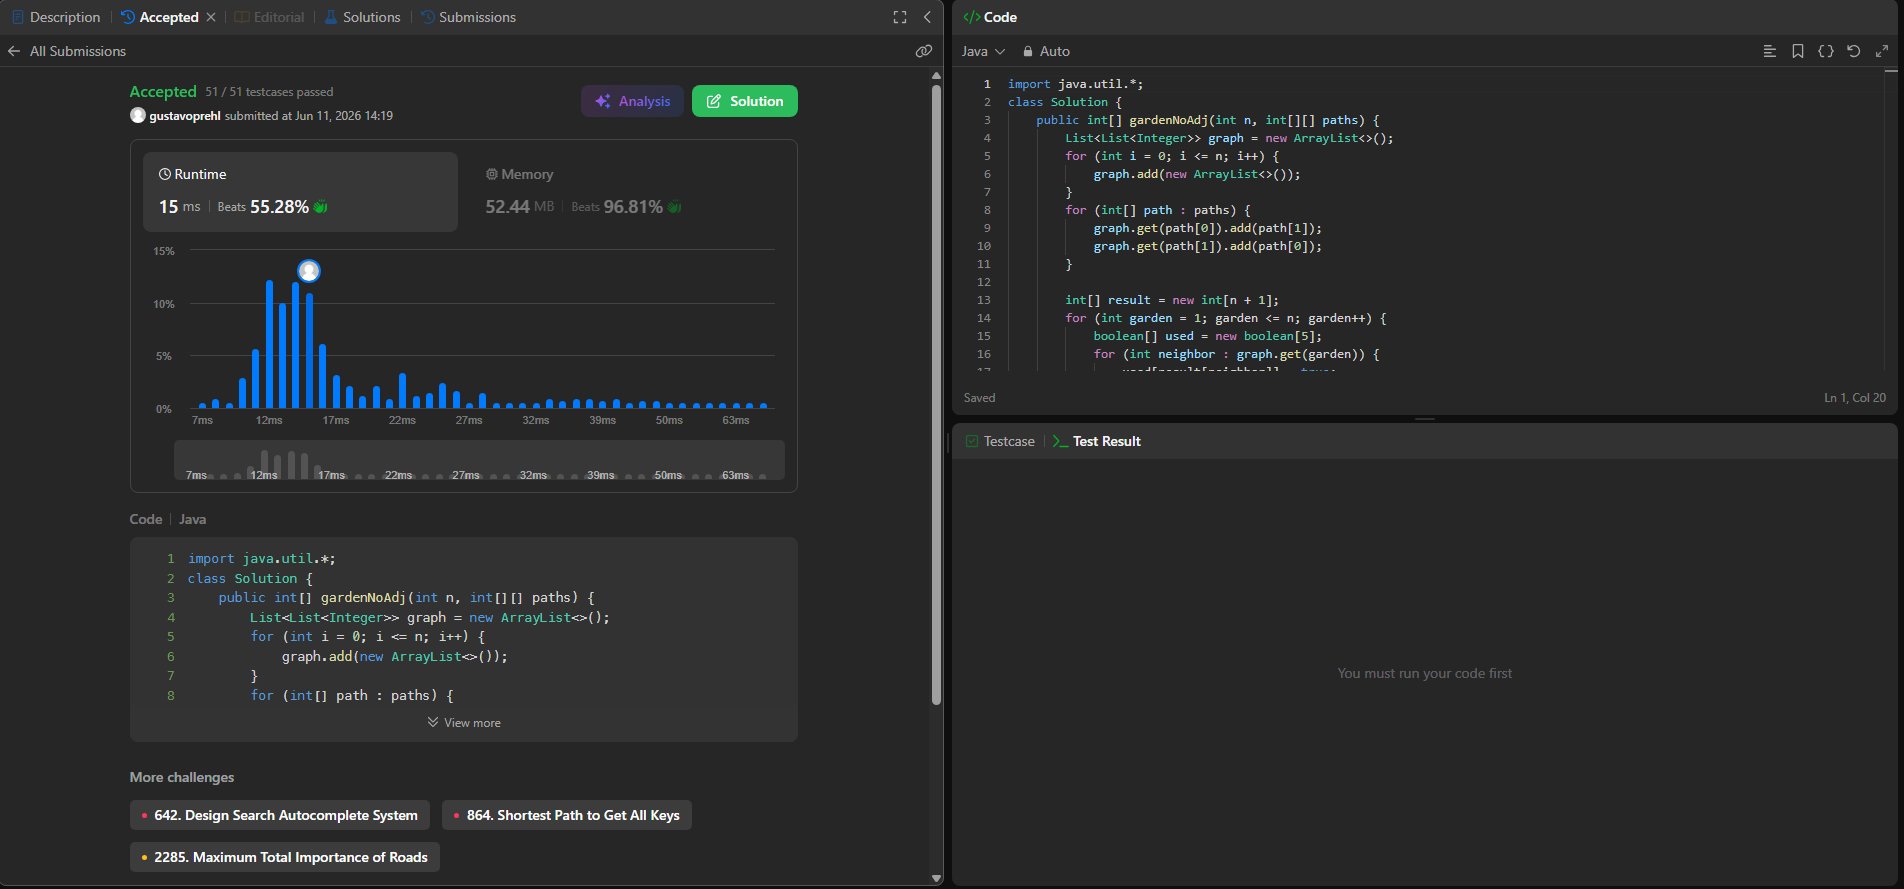
\includegraphics[width=0.85\textwidth]{Accepts/1042_FlowerPlanting_Submit.png}\\
\end{center}

\subsection*{Justificativa}

\textbf{Estratégia:} coloração gulosa de grafos.

O problema é equivalente a colorir os vértices de um grafo (jardins =
vértices, caminhos = arestas) de forma que vértices adjacentes recebam cores
diferentes, usando até 4 cores (tipos de flores).

\textbf{Por que 4 cores sempre bastam (correção):} a restrição garante que
cada vértice tem grau no máximo 3 (no máximo 3 caminhos incidentes). Pelo
teorema da coloração gulosa, qualquer grafo pode ser colorido com no máximo
$\Delta + 1$ cores, onde $\Delta$ é o grau máximo --- basta processar os
vértices em qualquer ordem e, para cada um, atribuir a menor cor que ainda
não foi usada por nenhum de seus vizinhos já coloridos. Como
$\Delta \leq 3$, sempre haverá pelo menos uma cor livre entre as 4
disponíveis, mesmo que todos os vizinhos já coloridos usem cores distintas
entre si.

\textbf{Implementação:} constrói-se a lista de adjacência a partir de
\texttt{paths} e, para cada jardim de 1 a $n$, marca-se em um vetor booleano
\texttt{used[1..4]} quais cores já foram usadas pelos vizinhos processados
anteriormente; a primeira cor livre é atribuída ao jardim atual.

\textbf{Complexidade:}
\begin{itemize}
    \item Tempo: $O(n + |paths|)$ --- a construção do grafo é $O(|paths|)$ e
    a coloração visita cada vértice e cada aresta um número constante de
    vezes (grau $\leq 3$).
    \item Espaço: $O(n + |paths|)$ para a lista de adjacência e o vetor de
    resultado.
\end{itemize}

\textbf{Tópico do curso:} coloração gulosa baseada no teorema $\Delta + 1$
--- \emph{Estratégia Gulosa e Divisão e Conquista} [CLRS09, caps. 4 e 16].
Como o algoritmo resolve o problema em tempo polinomial $O(n + |paths|)$, ele
também ilustra a \emph{Classe P} [CLRS09, cap. 34.1].

\newpage
\section{3286 --- Find a Safe Walk Through a Grid (LeetCode)}

\subsection*{Código}
\lstinputlisting{3286_FindSafeWalk.java}

\subsection*{Comprovante de aceite}
\begin{center}
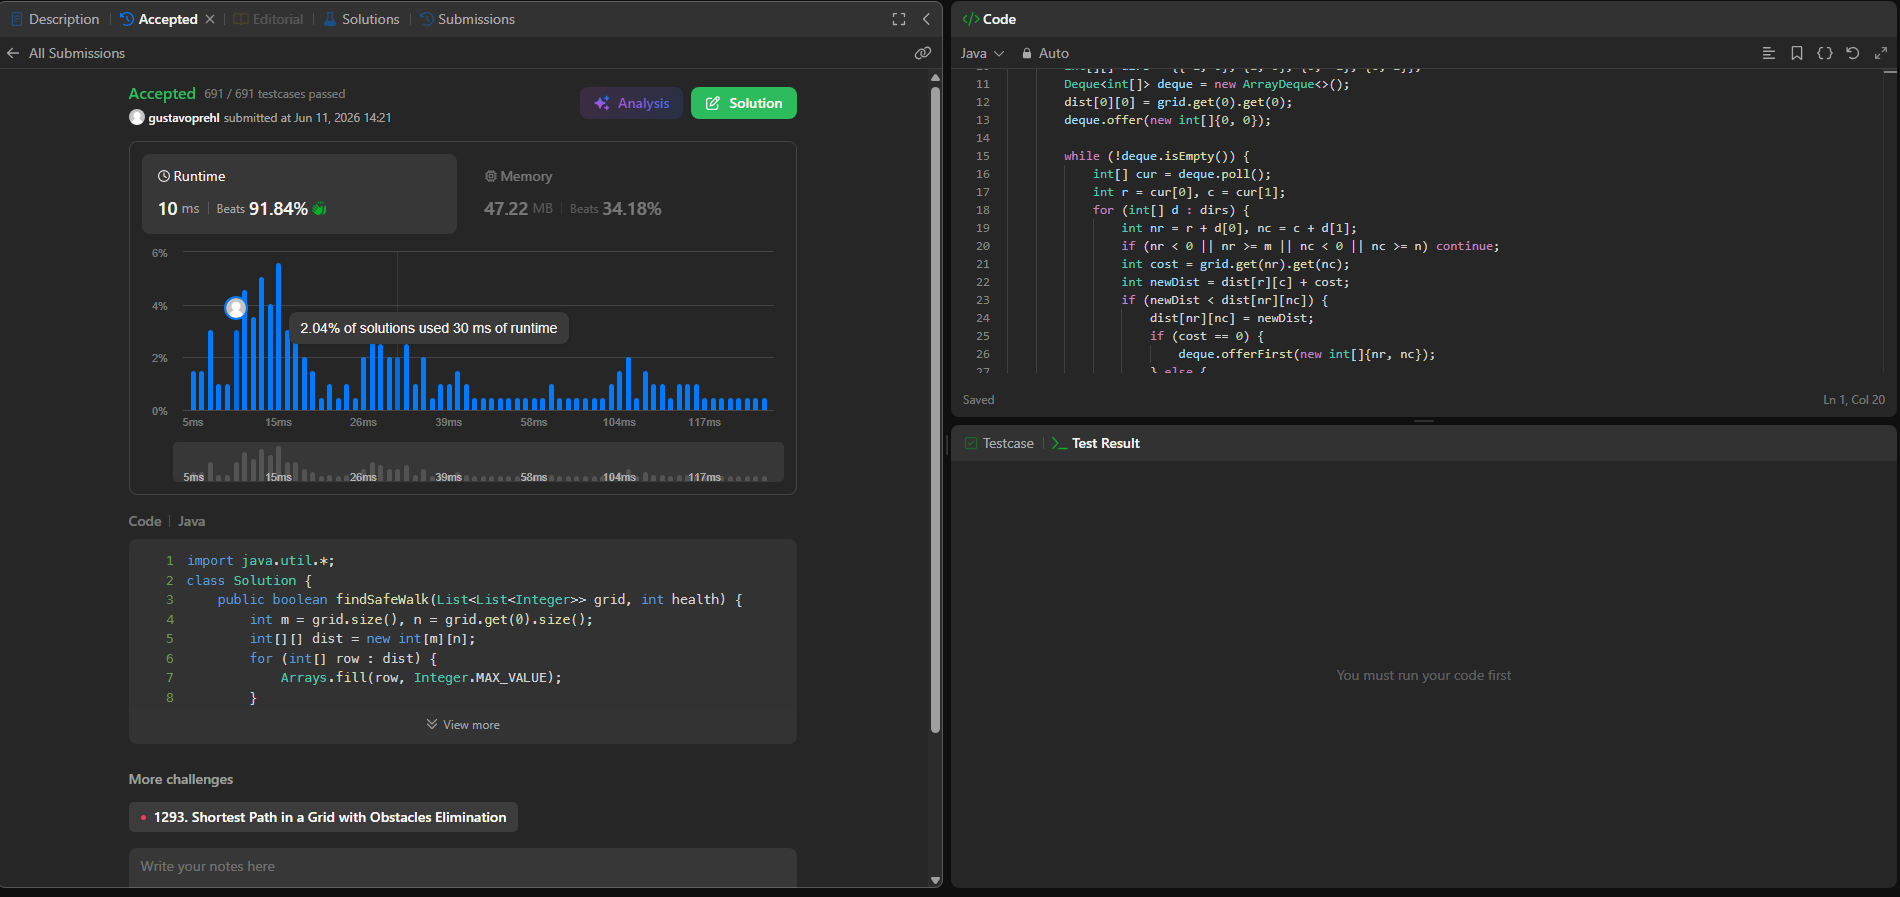
\includegraphics[width=0.85\textwidth]{Accepts/3286_FindSafeWalk_Submit.png}\\
\end{center}

\subsection*{Justificativa}

\textbf{Estratégia:} caminho mínimo em grafo com pesos $\{0, 1\}$ ---
algoritmo \textbf{0-1 BFS}, uma especialização do algoritmo de Dijkstra.

\textbf{Modelagem:} cada célula da grade é um vértice; há uma aresta entre
células adjacentes (4 direções). O ``custo'' de entrar em uma célula
\texttt{grid[i][j] = 1} é 1 (perde-se 1 ponto de vida) e o custo de uma
célula \texttt{grid[i][j] = 0} é 0. Definimos \texttt{dist[i][j]} como o
menor número total de células inseguras percorridas (incluindo a célula de
partida) em qualquer caminho de $(0,0)$ até $(i,j)$. A resposta é
\texttt{true} se e somente se \texttt{dist[m-1][n-1] <= health - 1}, ou seja,
se a vida restante ao chegar no destino for pelo menos 1.

\textbf{Por que o 0-1 BFS é correto (relação com Dijkstra):} o algoritmo de
Dijkstra processa vértices em ordem não decrescente de distância, garantindo
que, quando um vértice é retirado da estrutura, sua distância já é a
definitiva (propriedade da escolha gulosa + relaxamento de arestas). Como
aqui os pesos das arestas são apenas 0 ou 1, um deque substitui a fila de
prioridade: ao relaxar uma aresta de peso 0, o vizinho é inserido no início
do deque (mesma ``camada'' de distância); ao relaxar uma aresta de peso 1, o
vizinho é inserido no final (próxima camada). Essa invariante mantém o deque
sempre ordenado por distância, preservando a propriedade de Dijkstra sem
necessidade de heap.

\textbf{Complexidade:}
\begin{itemize}
    \item Tempo: $O(m \cdot n)$, pois cada célula é inserida/relaxada um
    número constante de vezes (grau $\leq 4$).
    \item Espaço: $O(m \cdot n)$ para a matriz \texttt{dist} e o deque.
\end{itemize}

\textbf{Tópico do curso:} a escolha gulosa de sempre expandir primeiro o
vértice de menor distância provisória (garantida pela ordenação do deque no
0-1 BFS) é a mesma propriedade de corretude do algoritmo de Dijkstra ---
\emph{Estratégia Gulosa e Divisão e Conquista} [CLRS09, caps. 4 e 16].

\newpage
\section{52 --- N-Queens II (LeetCode)}

\subsection*{Código}
\lstinputlisting{52_NQueensII.java}

\subsection*{Comprovante de aceite}
\begin{center}
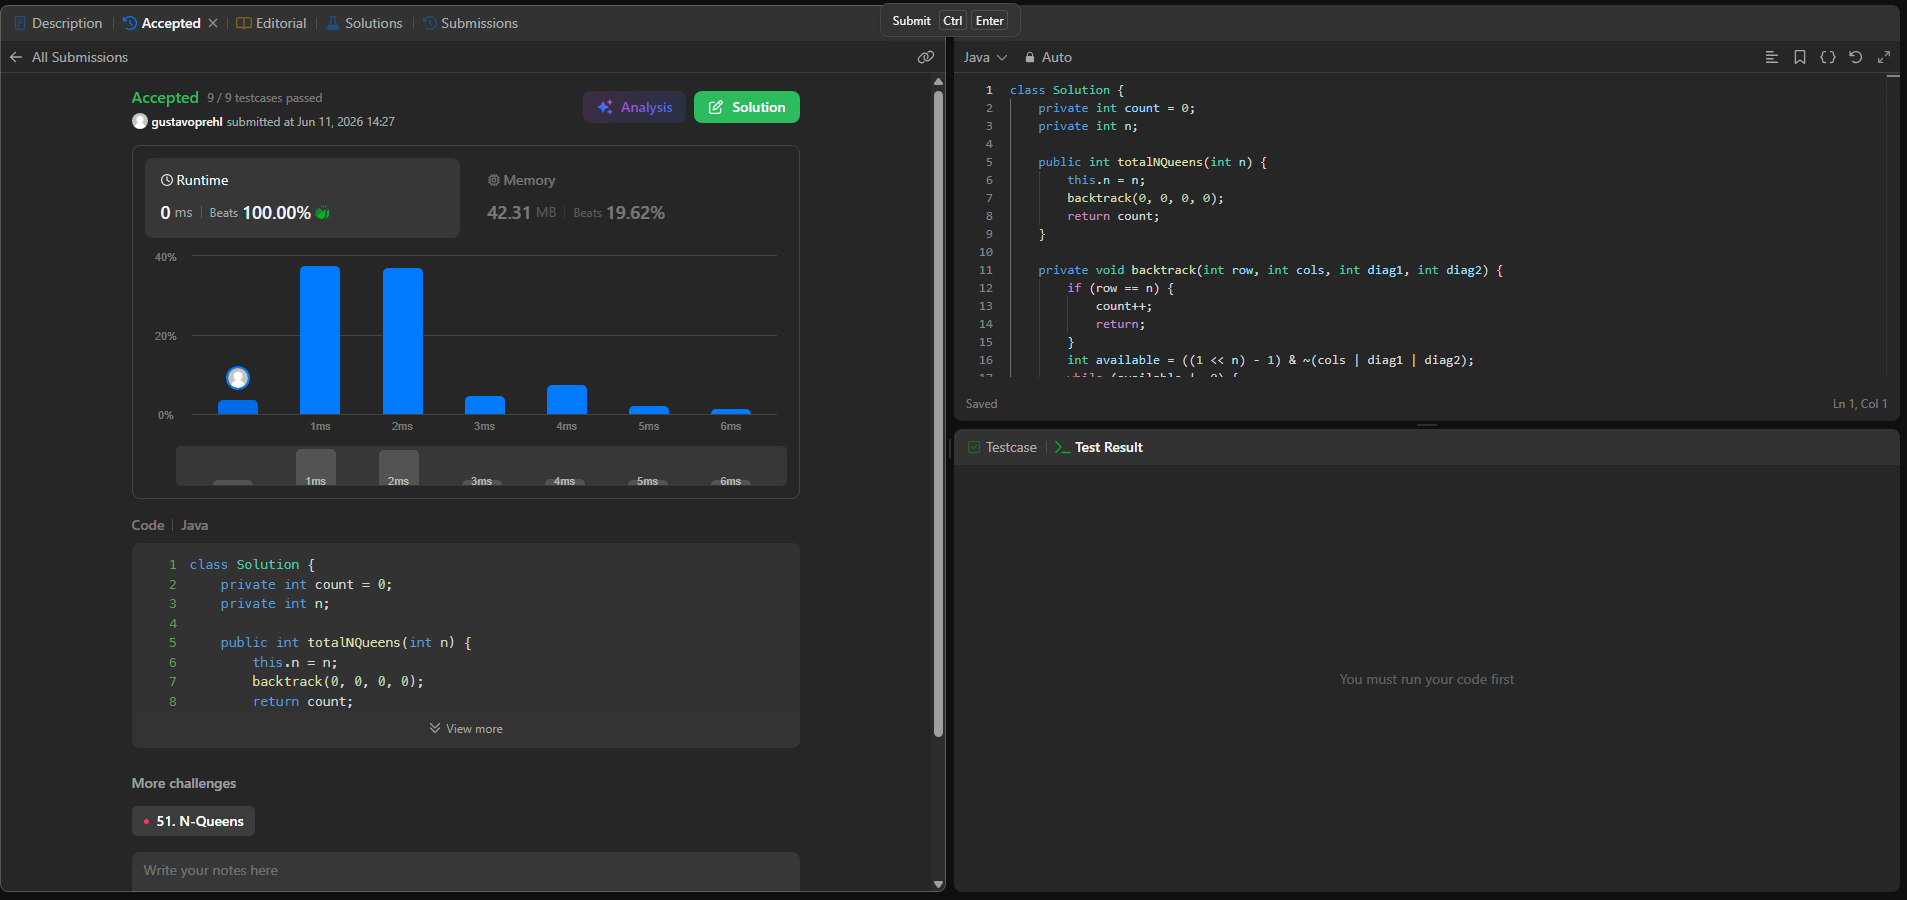
\includegraphics[width=0.85\textwidth]{Accepts/52_NQueensII_Submit.png}\\
\end{center}

\subsection*{Justificativa}

\textbf{Estratégia:} \emph{backtracking} (busca em profundidade no espaço de
soluções) com poda via \emph{bitmask}.

\textbf{Modelagem:} como duas rainhas nunca podem ficar na mesma linha, basta
decidir, para cada linha de $0$ a $n-1$, em qual coluna colocar a rainha
daquela linha. Isso reduz o espaço de busca de $2^{n^2}$ (todas as
combinações de casas) para no máximo $n^n$ (uma coluna por linha), e a poda
reduz ainda mais na prática.

\textbf{Representação por bitmask:} três inteiros guardam, em cada posição de
bit, se uma coluna (\texttt{cols}), uma diagonal principal (\texttt{diag1})
ou uma diagonal secundária (\texttt{diag2}) já está ``sob ataque'' pelas
rainhas colocadas até a linha atual. A operação
\texttt{((1 << n) - 1) \& \textasciitilde(cols | diag1 | diag2)} calcula em
$O(1)$ o conjunto de colunas livres para a linha atual.

\textbf{Poda (branch and bound):} ao avançar para a próxima linha,
atualiza-se \texttt{cols}, \texttt{diag1} (deslocada à esquerda) e
\texttt{diag2} (deslocada à direita) para refletir as novas casas atacadas.
Se, em alguma linha, \texttt{available == 0}, o ramo é descartado
imediatamente --- não há necessidade de continuar explorando colocações que
já violam as restrições do problema. Quando \texttt{row == n}, uma solução
válida completa foi encontrada e o contador é incrementado.

\textbf{Complexidade:}
\begin{itemize}
    \item Tempo: no pior caso $O(N!)$, mas a poda elimina a grande maioria
    dos ramos inválidos antes de chegar às últimas linhas (na prática, muito
    mais rápido que a enumeração ingênua).
    \item Espaço: $O(N)$ para a profundidade da recursão (não há estruturas
    adicionais de tamanho $O(N^2)$).
\end{itemize}

\textbf{Tópico do curso:} \emph{Branch-and-Bound e Backtracking} --- a busca
explora o espaço de soluções por profundidade e poda ramos inviáveis assim
que a inconsistência é detectada (\texttt{available == 0}), sem necessidade
de explorá-los até o fim.

\newpage
\section{2360 --- Longest Cycle in a Graph (LeetCode)}

\subsection*{Código}
\lstinputlisting{2360_LongestCycle.java}

\subsection*{Comprovante de aceite}
\begin{center}
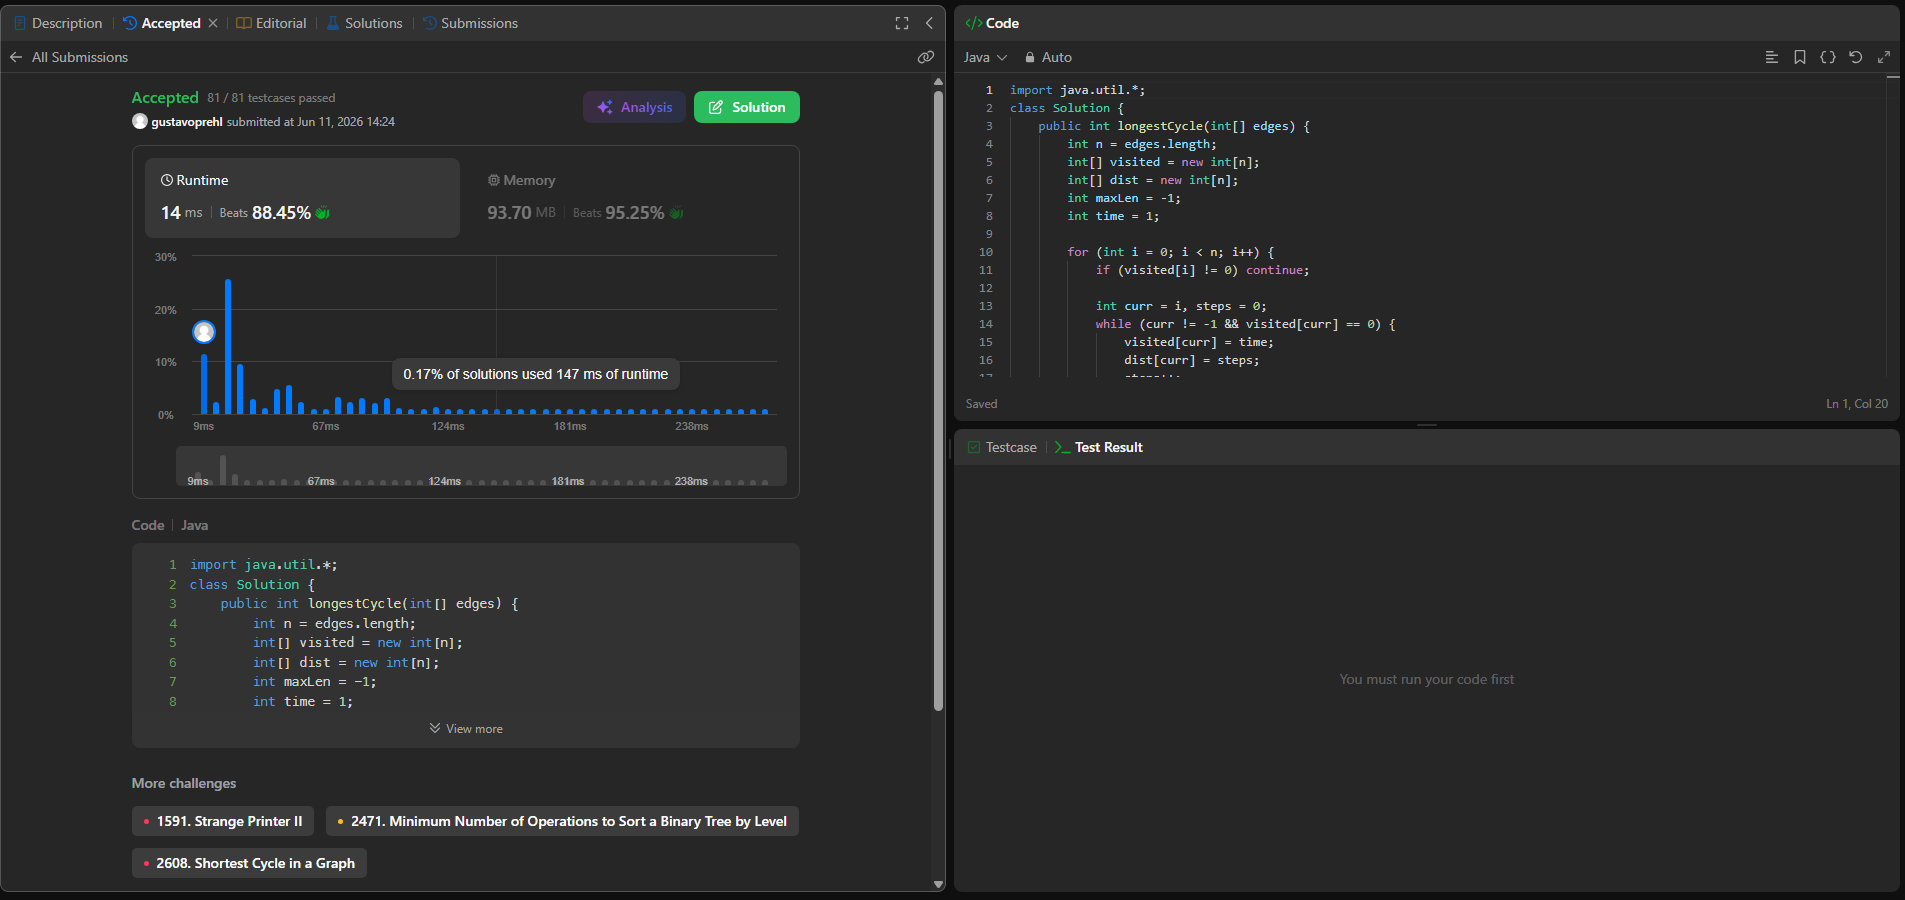
\includegraphics[width=0.85\textwidth]{Accepts/2360_LongestCycle_Submit.png}\\
\end{center}

\subsection*{Justificativa}

\textbf{Estratégia:} travessia iterativa de grafo funcional com marcação por
\emph{timestamp} (variação de busca em profundidade sem recursão/pilha
extra).

\textbf{Estrutura do problema:} como cada nó tem grau de saída no máximo 1, o
grafo é uma coleção de ``componentes funcionais'': cada um é uma cadeia de
nós que termina em $-1$ (sem ciclo) ou que eventualmente entra em um único
ciclo, em formato de $\rho$ (rho). Isso significa que, a partir de qualquer
nó, seguir os ponteiros \texttt{edges[i]} leva, no máximo, a um único ciclo.

\textbf{Algoritmo:} para cada nó \texttt{i} ainda não visitado, percorre-se a
cadeia a partir dele, atribuindo a cada nó visitado nessa travessia um
\texttt{timestamp} (identificador da travessia atual) e a sua distância
(\texttt{dist}, número de passos desde \texttt{i}). A travessia para quando:
\begin{itemize}
    \item chega a $-1$ (cadeia sem ciclo) --- não há ciclo a contabilizar; ou
    \item chega a um nó já visitado:
    \begin{itemize}
        \item se o \texttt{timestamp} desse nó for o \textbf{mesmo} da
        travessia atual, então o nó faz parte de um ciclo encontrado
        \textbf{agora}, e o tamanho do ciclo é
        \texttt{passos\_atuais - dist[nó]} (a diferença entre quando o nó
        foi ``reencontrado'' e quando foi visitado pela primeira vez nesta
        mesma travessia);
        \item se o \texttt{timestamp} for de uma travessia
        \textbf{anterior}, a cadeia atual apenas se conecta a um componente
        já processado, sem formar um novo ciclo.
    \end{itemize}
\end{itemize}

\textbf{Por que cada nó é processado uma única vez (correção da
complexidade):} uma vez que \texttt{visited[curr] != 0}, o nó nunca é
revisitado por outra travessia (a condição \texttt{visited[curr] == 0} no
laço \texttt{while} impede isso). Logo, cada nó é marcado e processado
exatamente uma vez ao longo de todas as travessias.

\textbf{Complexidade:}
\begin{itemize}
    \item Tempo: $O(n)$, pois cada nó é visitado uma única vez no total,
    somando todas as travessias.
    \item Espaço: $O(n)$ para os vetores \texttt{visited} e \texttt{dist}.
\end{itemize}

\textbf{Tópico do curso:} \emph{Análise de Algoritmos Iterativos} [CLRS09,
caps. 1 e 2.2] --- o algoritmo é estruturado como laços iterativos (sem
recursão), e o argumento de que cada nó é marcado e processado no máximo uma
vez é o que garante o limite $O(n)$ no total de iterações.

\newpage
\section{516 --- Longest Palindromic Subsequence (LeetCode)}

\subsection*{Código}
\lstinputlisting{516_LongestPalindromicSubsequence.java}

\subsection*{Comprovante de aceite}
\begin{center}
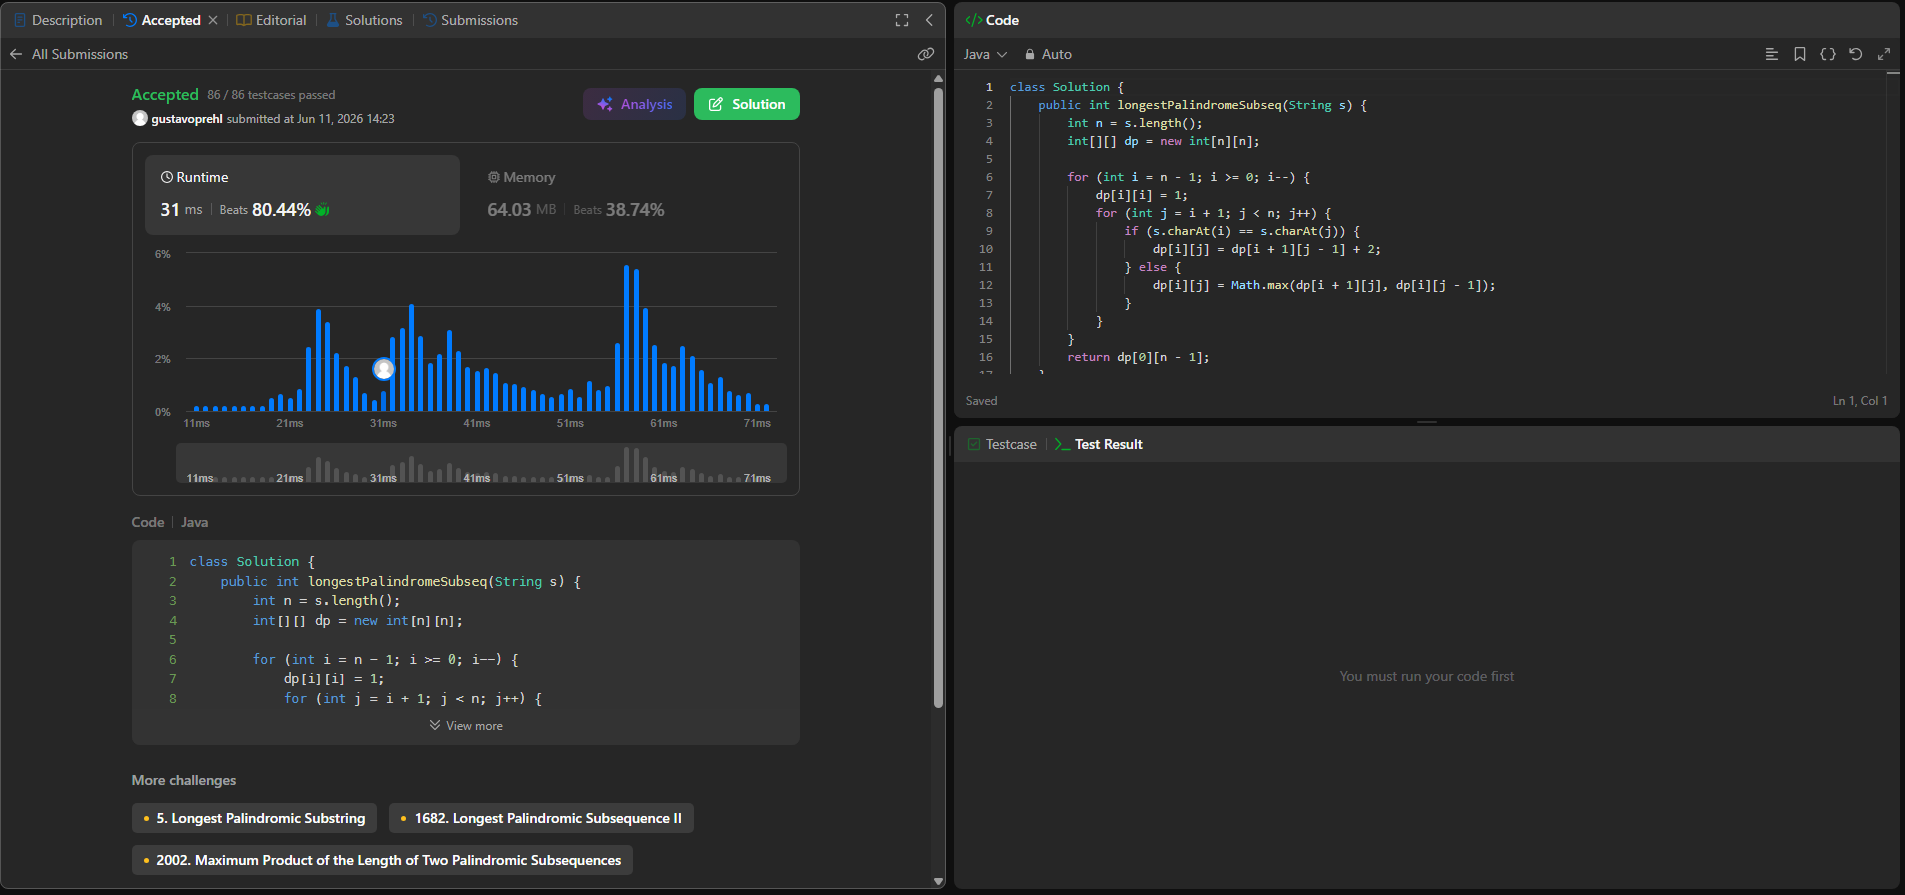
\includegraphics[width=0.85\textwidth]{Accepts/516_LongestPalindromicSubsequence_Submit.png}\\
\end{center}

\subsection*{Justificativa}

\textbf{Estratégia:} programação dinâmica em intervalos (\emph{interval
DP}).

\textbf{Definição do subproblema:} \texttt{dp[i][j]} representa o
comprimento da maior subsequência palíndroma contida em \texttt{s[i..j]}
(substring de \texttt{i} a \texttt{j}, inclusive).

\textbf{Subestrutura ótima (recorrência):} compara-se os caracteres das
extremidades do intervalo:
\begin{itemize}
    \item Se \texttt{s[i] == s[j]}, ambos os caracteres podem fazer parte da
    subsequência palíndroma (um na ponta esquerda, outro na direita), e o
    problema se reduz a encontrar a maior subsequência palíndroma do
    intervalo interno \texttt{s[i+1..j-1]}, somando 2:
    \texttt{dp[i][j] = dp[i+1][j-1] + 2}.
    \item Se \texttt{s[i] != s[j]}, pelo menos um dos dois extremos não pode
    pertencer à subsequência ótima, então a resposta é o melhor entre
    ignorar a extremidade esquerda ou a direita:
    \texttt{dp[i][j] = max(dp[i+1][j], dp[i][j-1])}.
\end{itemize}

\textbf{Caso base:} \texttt{dp[i][i] = 1}, pois um único caractere é sempre
um palíndromo de tamanho 1.

\textbf{Subproblemas sobrepostos e ordem de preenchimento:}
\texttt{dp[i][j]} depende apenas de subintervalos menores
(\texttt{dp[i+1][j-1]}, \texttt{dp[i+1][j]}, \texttt{dp[i][j-1]}), todos com
\texttt{i} maior ou \texttt{j} menor que o intervalo atual. Preenchendo
\texttt{i} de \texttt{n-1} até \texttt{0} e, para cada \texttt{i},
\texttt{j} de \texttt{i+1} até \texttt{n-1}, garante-se que toda dependência
já foi calculada antes de ser usada (programação dinâmica \emph{bottom-up}).

\textbf{Resposta final:} \texttt{dp[0][n-1]}, o intervalo que cobre a string
inteira.

\textbf{Complexidade:}
\begin{itemize}
    \item Tempo: $O(n^2)$, um valor para cada par $(i, j)$ com
    $i \leq j$.
    \item Espaço: $O(n^2)$ para a tabela \texttt{dp}.
\end{itemize}

\textbf{Tópico do curso:} \emph{Programação Dinâmica} [CLRS09, cap. 15] ---
formulação de \texttt{dp[i][j]} sobre intervalos da string, com recorrência
baseada em subintervalos menores e preenchimento \emph{bottom-up} respeitando
as dependências entre subproblemas.

\newpage
\section{1971 --- Find if Path Exists in Graph (LeetCode)}

\subsection*{Código}
\lstinputlisting{1971_FindIfPathExists.java}

\subsection*{Comprovante de aceite}
\begin{center}
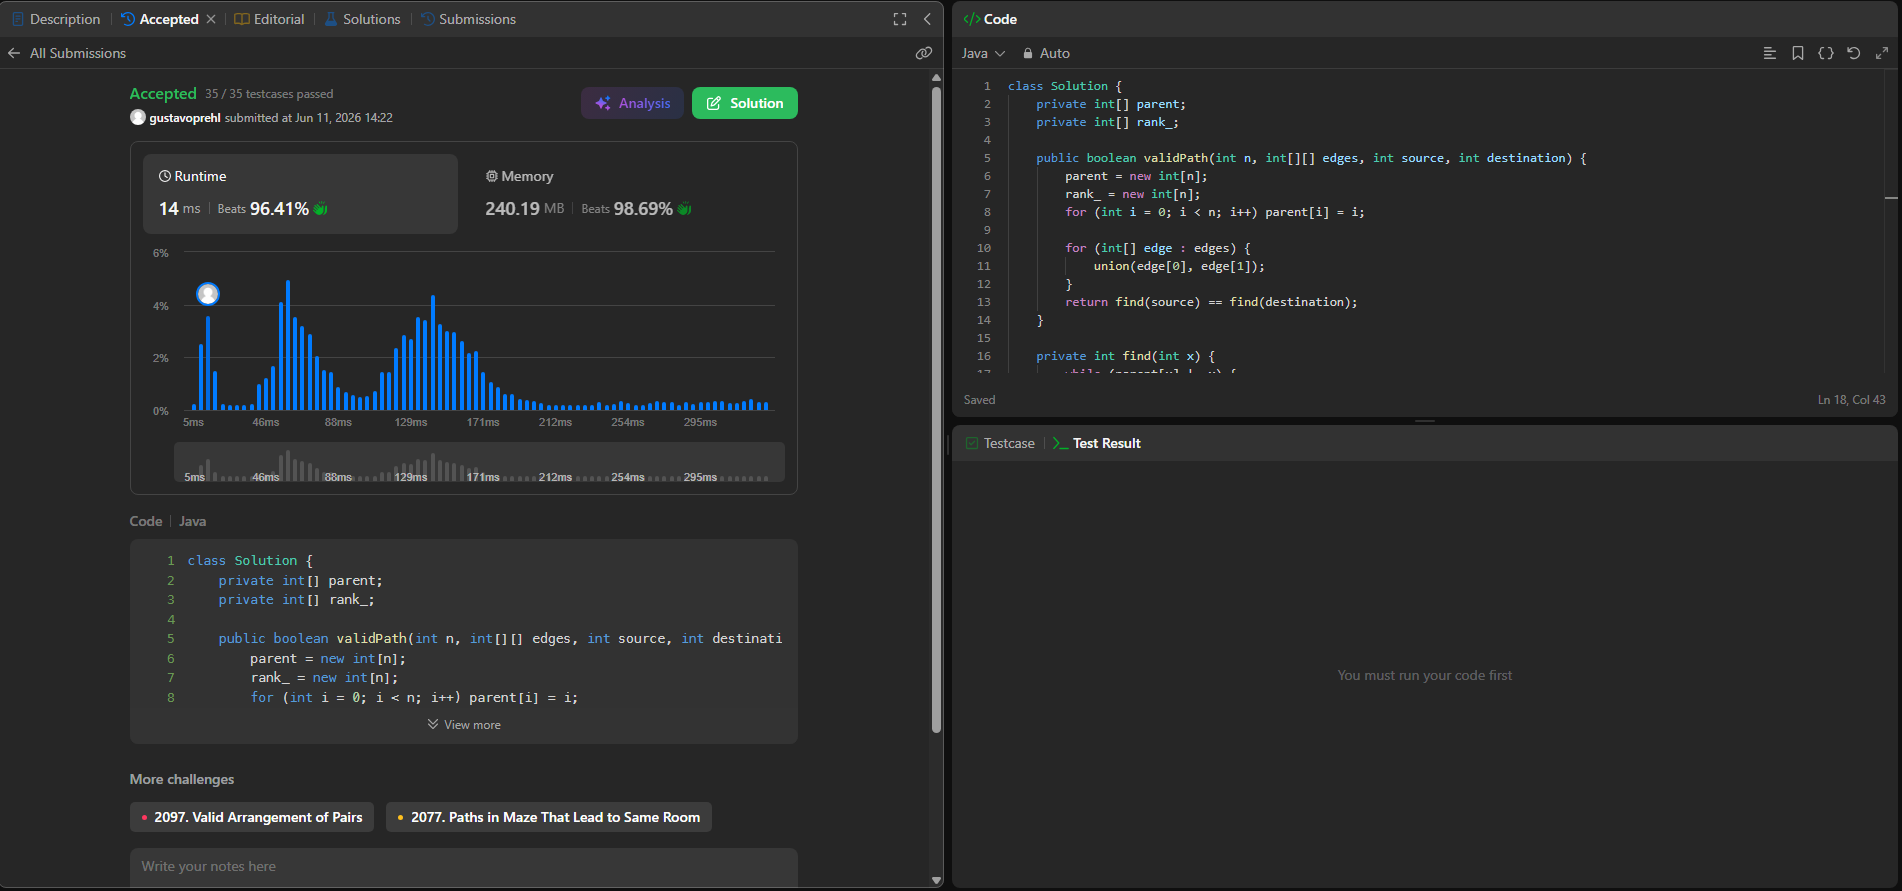
\includegraphics[width=0.85\textwidth]{Accepts/1971_FindIfPathExists_Submit.png}\\
\end{center}

\subsection*{Justificativa}

\textbf{Estratégia:} Union-Find (\emph{Disjoint Set Union} --- DSU) com
compressão de caminho e união por \emph{rank}.

\textbf{Modelagem:} existe um caminho entre \texttt{source} e
\texttt{destination} se e somente se os dois vértices pertencem ao mesmo
componente conexo do grafo. A estrutura DSU mantém uma partição dos vértices
em conjuntos disjuntos, onde cada conjunto representa um componente conexo,
identificado por um representante (raiz).

\textbf{Construção:} inicialmente cada vértice é seu próprio conjunto
(\texttt{parent[i] = i}). Para cada aresta \texttt{(u, v)} em \texttt{edges},
executa-se \texttt{union(u, v)}, unindo os conjuntos aos quais \texttt{u} e
\texttt{v} pertencem. Ao final, basta verificar se
\texttt{find(source) == find(destination)}.

\textbf{Compressão de caminho (\texttt{find}):} ao buscar a raiz de um
elemento, cada nó visitado é reconectado mais perto da raiz (aqui via
\emph{path halving}: \texttt{parent[x] = parent[parent[x]]}), achatando a
árvore e acelerando buscas futuras.

\textbf{União por rank (\texttt{union}):} ao unir dois conjuntos, a raiz da
árvore de menor \texttt{rank} (altura estimada) é pendurada na raiz da árvore
de maior \texttt{rank}, evitando que as árvores fiquem muito altas.

\textbf{Complexidade (teoria de DSU):} combinando compressão de caminho e
união por rank, cada operação \texttt{find}/\texttt{union} tem custo
amortizado $O(\alpha(n))$, onde $\alpha$ é a inversa da função de Ackermann
--- na prática, uma constante muito pequena ($\leq 4$ para qualquer $n$
razoável).

\begin{itemize}
    \item Tempo: $O((n + |edges|) \cdot \alpha(n)) \approx O(n + |edges|)$.
    \item Espaço: $O(n)$ para os vetores \texttt{parent} e
    \texttt{rank\_}.
\end{itemize}

\textbf{Tópico do curso:} a construção do DSU é puramente iterativa (laços
sobre os vértices e sobre \texttt{edges}), enquadrando-se em \emph{Análise de
Algoritmos Iterativos} [CLRS09, caps. 1 e 2.2]; como o tempo total é
quase-linear, $O((n+|edges|)\cdot\alpha(n))$, o algoritmo também é um exemplo
de problema na \emph{Classe P} [CLRS09, cap. 34.1].

\newpage
\section{654 --- Maximum Binary Tree (LeetCode)}

\subsection*{Código}
\lstinputlisting{654_MaximumBinaryTree.java}

\subsection*{Comprovante de aceite}
\begin{center}
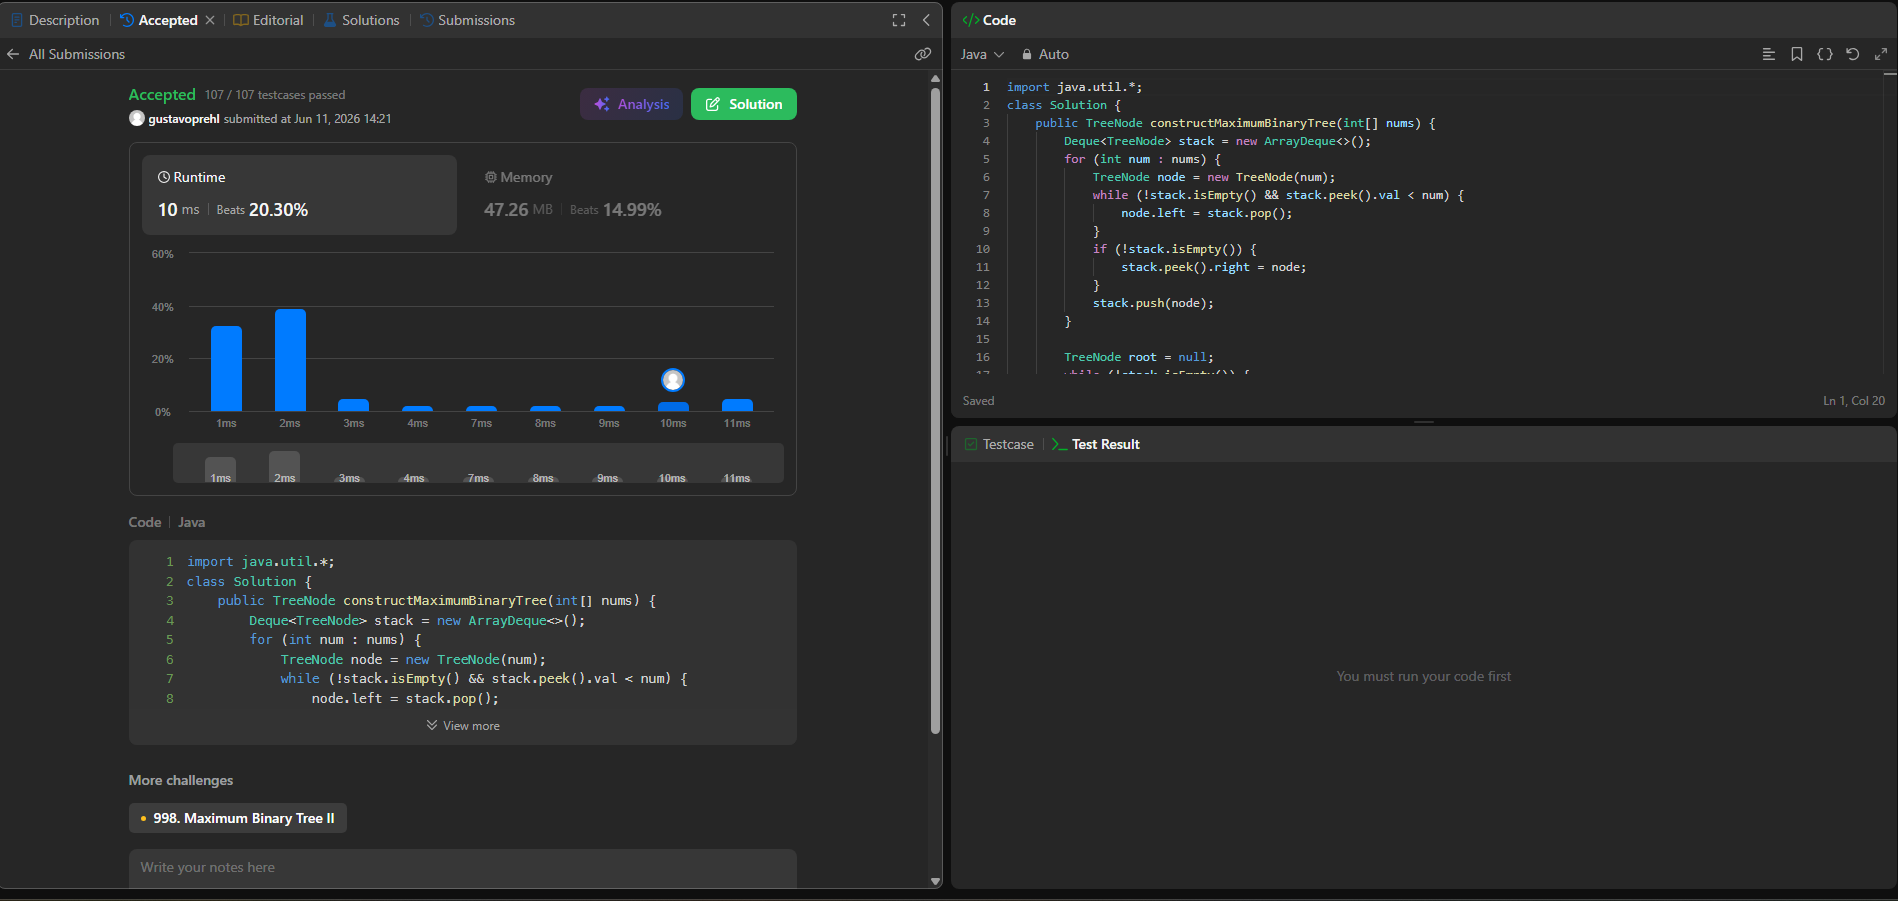
\includegraphics[width=0.85\textwidth]{Accepts/654_MaximumBinaryTree_Submit.png}\\
\end{center}

\subsection*{Justificativa}

\textbf{Estratégia:} pilha monotônica, construindo a árvore em uma única
passagem (em vez da abordagem ingênua $O(n^2)$ de buscar o máximo de cada
subarray recursivamente).

\textbf{Invariante da pilha:} a pilha mantém, do fundo para o topo, os nós
que ainda não encontraram, à sua direita, um valor maior que o seu --- ou
seja, candidatos a serem ``dominados'' por um número futuro. Os valores na
pilha são estritamente decrescentes do fundo para o topo, e cada nó é o
filho direito do nó imediatamente abaixo dele (formando a ``espinha
direita'' da árvore parcial construída até o momento).

\textbf{Relação com a definição recursiva do problema:} na árvore binária
máxima, o pai de um elemento \texttt{nums[i]} é o \textbf{menor} entre o
primeiro elemento maior à sua esquerda e o primeiro elemento maior à sua
direita (o ``dominador'' mais próximo). Ao processar \texttt{nums} da
esquerda para a direita:
\begin{itemize}
    \item Se o número atual é \textbf{maior} que o topo da pilha, ele é o
    primeiro elemento maior à direita de todos os nós removidos --- portanto,
    o número atual se torna ancestral deles. O último nó removido (o de
    maior valor entre os removidos, e portanto o mais próximo na hierarquia)
    vira o \textbf{filho esquerdo} do novo nó; os demais já estavam
    encadeados como filhos direitos uns dos outros, preservando a ordem
    relativa original.
    \item Se a pilha não ficou vazia após as remoções, o topo restante é o
    primeiro elemento maior à esquerda do número atual --- logo, o número
    atual se torna \textbf{filho direito} desse nó.
\end{itemize}

\textbf{Análise amortizada (custo $O(n)$):} cada elemento de \texttt{nums} é
empilhado exatamente uma vez e desempilhado no máximo uma vez durante toda a
execução. Pelo método agregado de análise amortizada, o número total de
operações de pilha (\emph{push} + \emph{pop}) ao longo das $n$ iterações é,
no máximo, $2n$, mesmo que o laço \texttt{while} interno execute múltiplas
vezes em iterações específicas.

\textbf{Complexidade:}
\begin{itemize}
    \item Tempo: $O(n)$ amortizado.
    \item Espaço: $O(n)$ para a pilha (no pior caso, array estritamente
    crescente).
\end{itemize}

\textbf{Tópico do curso:} a definição do problema --- o pai de cada elemento
é o menor entre os ``dominadores'' à esquerda e à direita --- corresponde a
uma formulação recursiva de divisão e conquista (\emph{Estratégia Gulosa e
Divisão e Conquista} [CLRS09, caps. 4 e 16]); a implementação com pilha
monotônica é a versão iterativa otimizada dessa recursão, cuja análise de
custo amortizado $O(n)$ se enquadra em \emph{Análise de Algoritmos
Iterativos} [CLRS09, caps. 1 e 2.2].

\newpage
\section{E --- The Lakes (Codeforces)}

\subsection*{Código}
\lstinputlisting{E_TheLakes/Main.java}

\subsection*{Comprovante de aceite}
\begin{center}
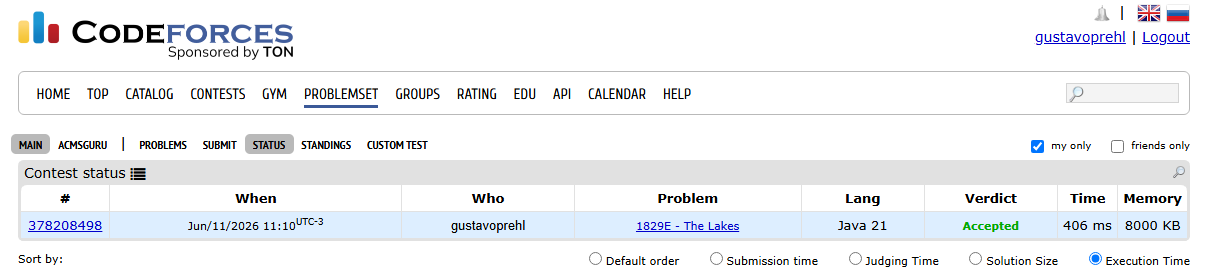
\includegraphics[width=0.85\textwidth]{Accepts/E_TheLakes.png}
\end{center}

\subsection*{Justificativa}

\textbf{Estratégia:} componentes conexas em grade (BFS), com leitura rápida e
fila explícita por questões de desempenho.

\textbf{Modelagem:} cada célula com \texttt{a[i][j] > 0} é um vértice de um
grafo implícito, com arestas para os vizinhos ortogonais (cima, baixo,
esquerda, direita) que também tenham valor $> 0$. Um ``lago'' é exatamente
uma componente conexa desse grafo, e seu ``volume'' é a soma dos valores dos
vértices da componente. O problema pede o maior volume entre todas as
componentes --- ou 0 se não existir nenhuma célula com valor $> 0$.

\textbf{Algoritmo:} percorre-se cada célula da grade; se ainda não foi
visitada e tem valor $> 0$, executa-se uma BFS a partir dela, somando os
valores de todas as células alcançadas (marcando-as como visitadas para não
serem reprocessadas). O maior valor de soma encontrado entre todas as BFS é
a resposta.

\textbf{Por que BFS iterativa com array em vez de DFS recursiva:} como
$n, m \leq 1000$ e a soma de $n \cdot m$ pode chegar a $10^6$, uma única
componente pode ter até $10^6$ células. Uma DFS recursiva nesse cenário
atingiria profundidade de recursão da ordem de $10^6$, estourando a pilha de
chamadas (\texttt{StackOverflowError}). A BFS com fila implementada como
array de tamanho \texttt{n*m} evita esse problema, processando cada célula em
$O(1)$ amortizado.

\textbf{Por que leitura rápida (\texttt{StreamTokenizer}):} com
$t \leq 10^4$ casos de teste e soma de $n \cdot m \leq 10^6$, o volume total
de números a serem lidos pode chegar à ordem de milhões. \texttt{Scanner} é
lento demais para essa escala (risco de \emph{Time Limit Exceeded});
\texttt{StreamTokenizer} sobre um \texttt{BufferedReader} realiza a
tokenização de forma eficiente, em tempo linear no tamanho da entrada.

\textbf{Complexidade (por caso de teste):}
\begin{itemize}
    \item Tempo: $O(n \cdot m)$ --- cada célula é visitada e processada uma
    única vez.
    \item Espaço: $O(n \cdot m)$ para os vetores \texttt{a},
    \texttt{visited} e \texttt{queue}.
\end{itemize}

Como a soma de $n \cdot m$ sobre todos os casos de teste é limitada a
$10^6$, o tempo total do programa é $O(10^6)$, dentro do limite de 3
segundos.

\textbf{Tópico do curso:} o algoritmo é descrito inteiramente por laços
iterativos (BFS com fila explícita e leitura via \texttt{StreamTokenizer}),
conforme \emph{Análise de Algoritmos Iterativos} [CLRS09, caps. 1 e 2.2]; sua
complexidade $O(n \cdot m)$ por caso de teste, linear no tamanho da entrada,
é o tipo de cota que caracteriza problemas tratáveis na \emph{Classe P}
[CLRS09, cap. 34.1].


\end{document}
